% chercher des documents LaTeX dans styles, corps et bib
\makeatletter\def\input@path{{styles/}{corps/}{bib/}}\makeatother


\documentclass[12pt, openany]{report}
\usepackage[a4paper,vdivide={*,22cm,4cm}]{geometry}
\usepackage[french]{babel}
\selectlanguage{french}
\usepackage[T1]{fontenc}
\usepackage[utf8]{inputenc}
\usepackage{pageGardeEnsta}
\usepackage{lmodern}
\usepackage{enumitem}
\usepackage{subcaption}
\usepackage{hyperref}
% pour charger des images
\usepackage{graphicx}
% répertoire dans lequel trouver les images
\graphicspath{{imgs/}}
% liens hypertexte dans le document
\usepackage[colorlinks,breaklinks]{hyperref}
\setlength{\parindent}{0pt}
\usepackage{float}
\usepackage{hyperref}
\usepackage{listings}
\usepackage[round]{natbib}
\usepackage{appendix}

\title{Véhicule autonome \\ suiveur de lignes}
\author{Colin Baumgard, Ludovic Diguet, Hamid Hacene, Corentin Lemoine, Antonin Lizé}
\date{\today}
\doctype{Middleware}
\promo{UE 4.1}
\etablissement{\textsc{Ensta} Bretagne\\2, rue François Verny\\
  29806 \textsc{Brest} cedex\\\textsc{France}\\Tel +33 (0)2 98 34 88 00\\ \url{www.ensta-bretagne.fr}}
\logoEcole{\includegraphics[height=4.2cm]{logo_ENSTA_Bretagne_Vertical_CMJN}}
\imgGarde{\centering\includegraphics[scale=0.4]{result.png}}

\renewcommand{\thesection}{\arabic{section}}
\begin{document}
\maketitle
\tableofcontents
\pagebreak

\section*{Introduction} 
\addcontentsline{toc}{chapter}{Introduction}
Ce projet s'inscrit dans le cadre des enseignements de l'\textsc{ENSTA Bretagne} dispensés aux élèves de deuxième année de la filière \textit{Robotique Autonome} au sein de l'U.E 4.1 : \textit{Middleware}.\\

<<<<<<< HEAD
Ce rapport présente le travail effectué par l’équipe "La CJC ROS". La répartition du travail au sein du groupe peut être retrouvée sur le dépôt git à l’adresse suivante : \href{https://github.com/HamidHacene/laCJC_ROS}{la CJC}\footnote{https://github.com/HamidHacene/laCJC\_ROS}.\\
=======
L'objectif est d'utiliser des connaissances acquises au long de l'année pour réaliser un projet robotique concret. Ce projet permet de toucher à de nombreux domaines : CAO et conception mécanique, éléctronique, OS, réseau, conception logiciel, OpenCV... De plus, travailler sur un même code en groupe  n'est pas évident, il est donc important de s'y former.

\section*{Abstract}
\addcontentsline{toc}{chapter}{Abstract}
In this article presents the realisation of an autonaumous 1:10 scale car. We will particularly talk about the software implementation. We have achied our goal using a rpi board and a camera and OpenCV to process images. ROS is used to have a modular code.

\pagebreak
>>>>>>> b5d2ff851ae198be8a7444f66db44fb074a962ed

\section{Présentation du projet}
\subsection{Problématique}
Nous avons pu acquérir au fil du semestre quatre une connaissance théorique et pratique du \textit{Middleware} \textsc{ROS} (Robot Operating System). Pour rappel, un \textit{Middleware} est un outil qui permet d'échanger des informations entre différentes applications et programmes via des techniques et des messages standardisés. \textsc{ROS} est un \textit{Middleware} développé par l'\textsc{Open Robotics}.\\

Le but de ce projet au sein de l'U.E est de maîtriser les concepts fondamentaux de \textsc{ROS} et d'arriver à les implémenter sur un robot. Il s'agit d'appliquer une démarche d'ingénierie afin de proposer des solutions adéquates en prenant en compte les différentes dimensions techniques du problème : \textit{hardware} et \textit{software}.\\

La problématique de départ se résume ainsi à "rendre un véhicule autonome pour accomplir un tour complet de la piste d'athlétisme de l'école". Les véhicules mis à disposition sont des voitures à l'échelle $1/10^ème$ construites par différents groupes au semestre précédent.

\begin{figure}[!h]
     \centering
     \begin{subfigure}[b]{0.45\textwidth}
         \centering
         \includegraphics[width=\textwidth, height = 5cm]{terrain.jpg}
         \caption{Terrain de l'\textit{ENSTA Bretagne}}
     \end{subfigure}
     ~
     \begin{subfigure}[b]{0.45\textwidth}
         \centering
         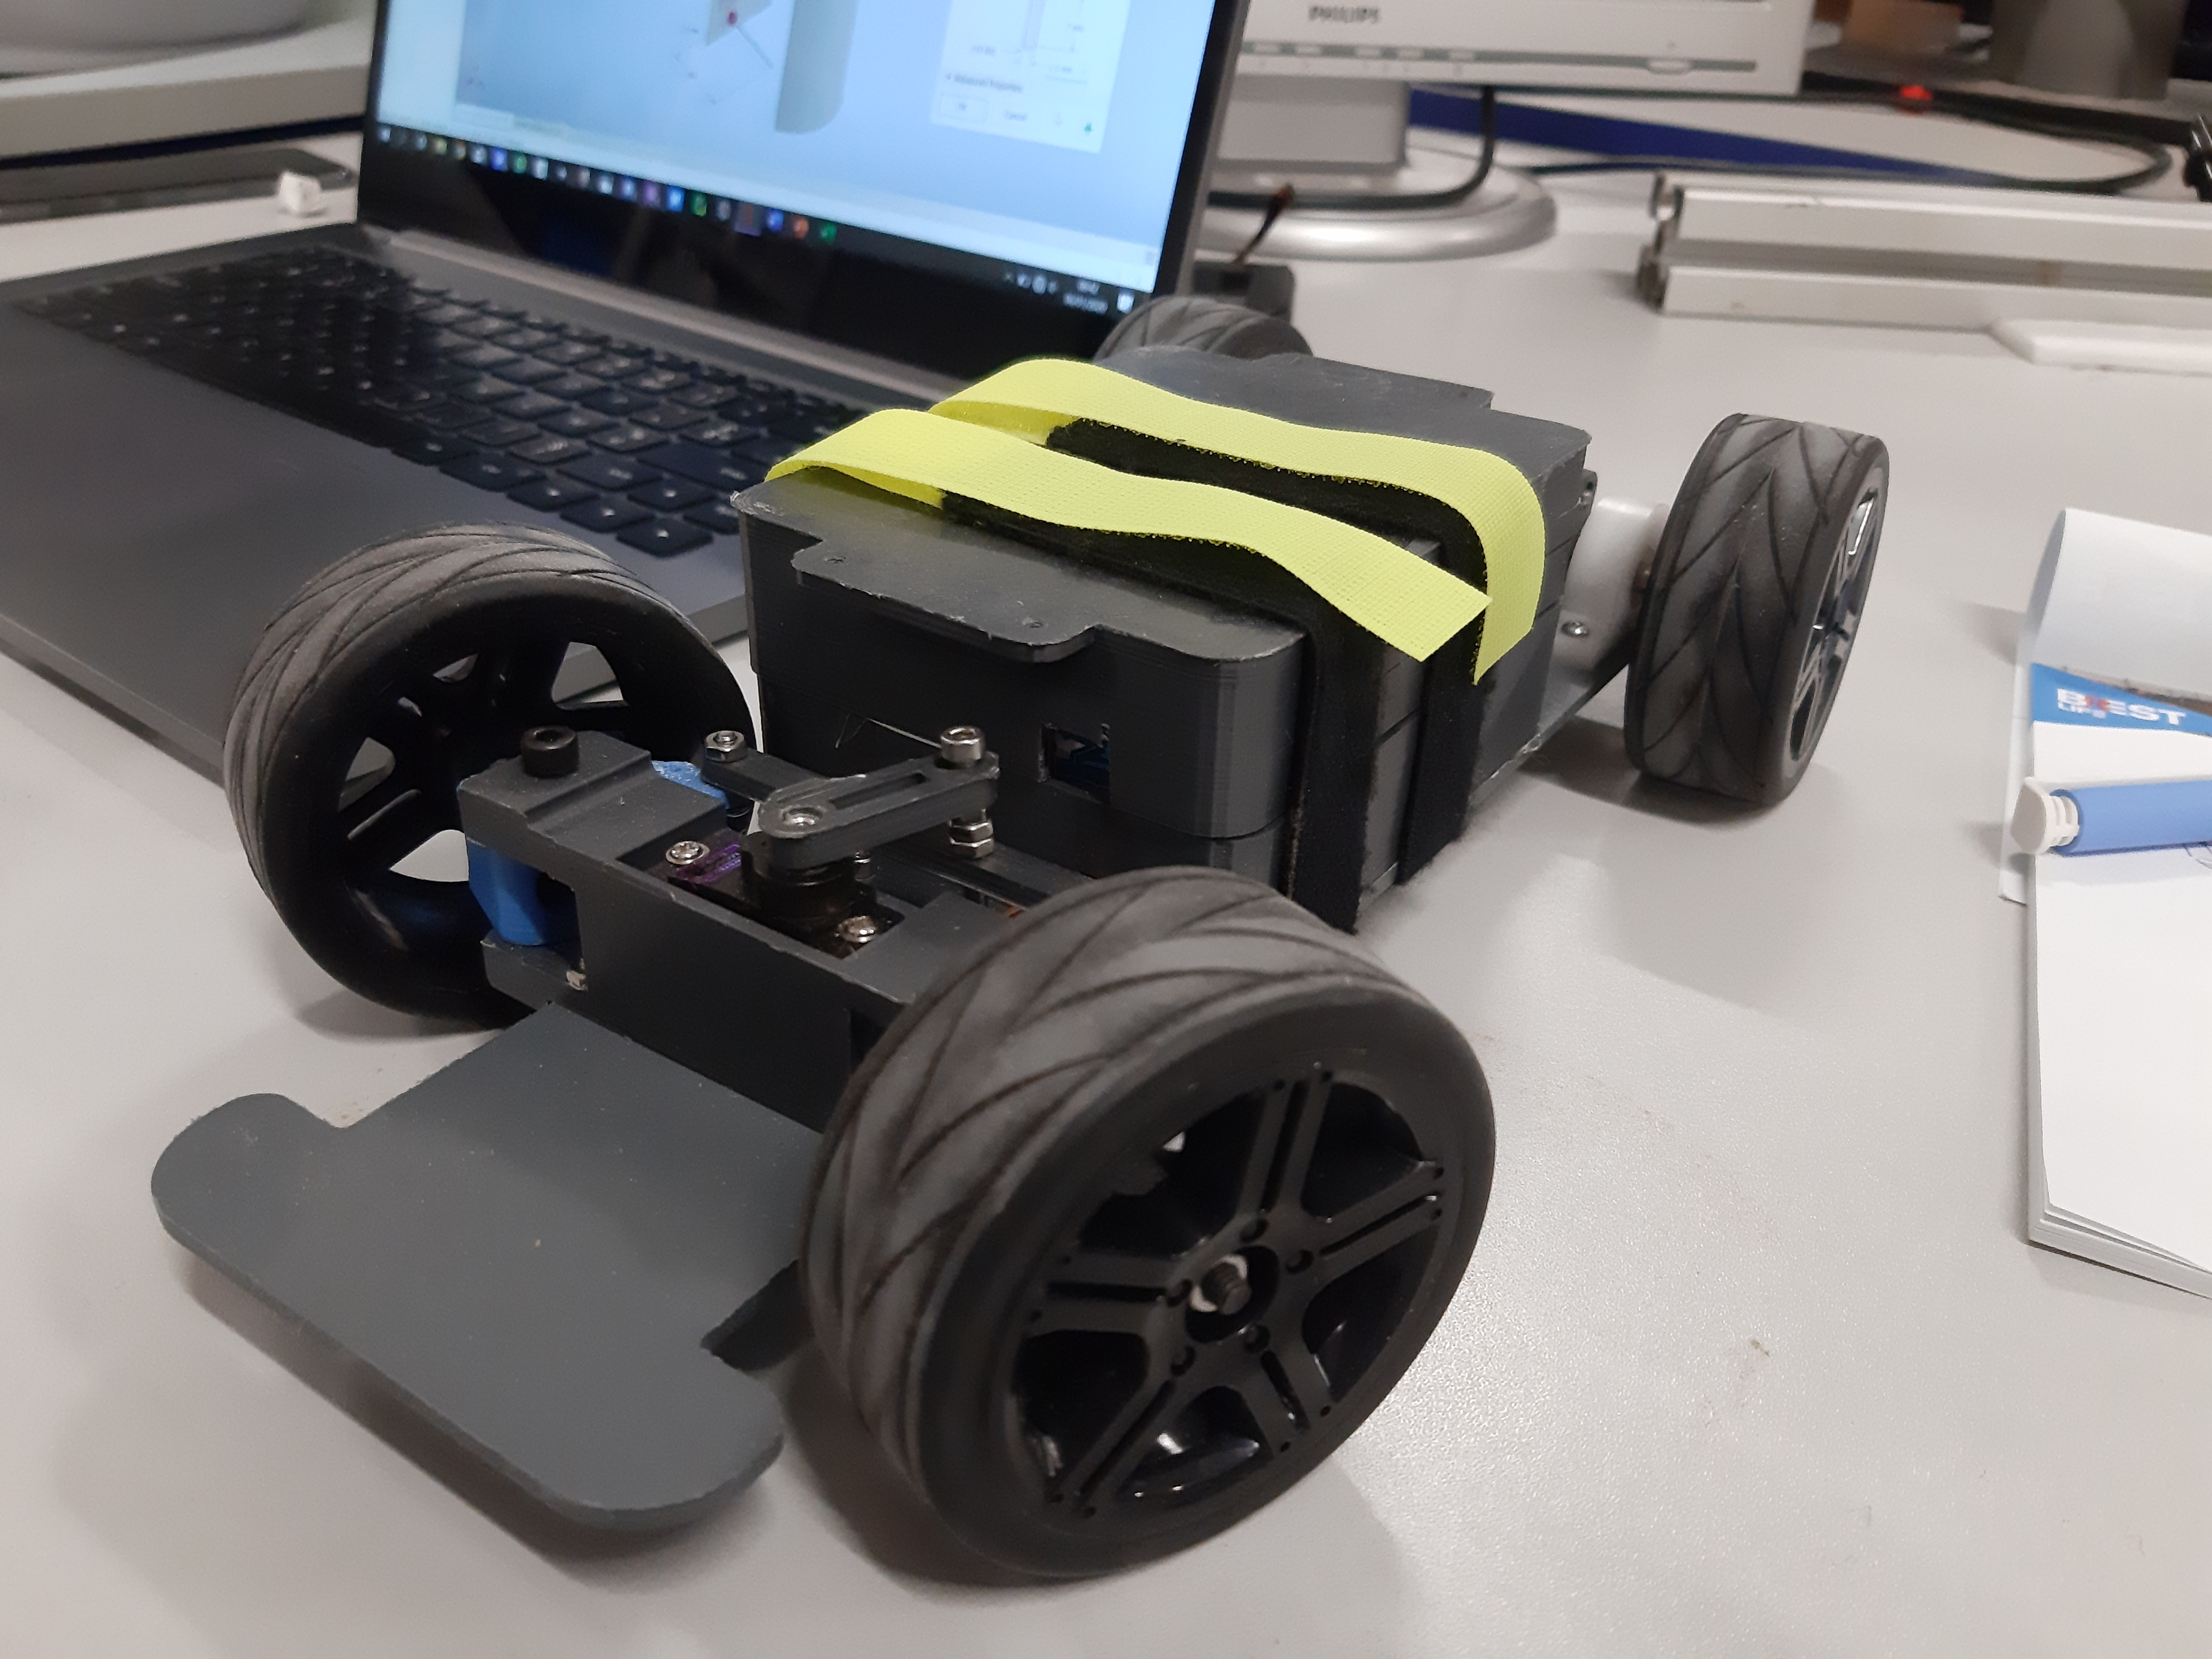
\includegraphics[width=\textwidth, height = 5cm]{voiture.jpg}
         \caption{Voiture utilisée pour le projet}
     \end{subfigure}
     \caption{Problématique du projet}
     \label{fig:prob}
\end{figure}

\subsection{Objectifs}
L'objectif principal de notre équipe est de répondre à la problématique tout en proposant une approche différente des autres groupes pour apporter une diversité aux contenus des projets.\\

Ainsi, nous nous sommes fixé ces trois objectifs supplémentaires : 
\begin{itemize}[label=\textbullet, font=\small]
    \item Proposer une approche réaliste qui s'inspire des voitures autonomes existantes sur le marché ou en développement ;
    \item Développer essentiellement en \textsc{C++} pour garantir la portabilité des algorithmes et l'implémentation sur d'autres structures ;\\
    \item Utiliser le plus possible les solutions et algorithmes proposés dans les \textit{packages} \textsc{ROS} afin d'exploiter au maximum les possibilités offertes par ce \textit{Middleware}.\\
\end{itemize}

Compte tenu de l'évolution de la pandémie du \textit{Covid-19}, et suite à la fermeture de l'\textit{ENSTA Bretagne}, nous avons revu la problématique et les objectifs du projets. À cause d'une avarie de matériel, l'objectif principal ne peut être atteint : il s'agit désormais de construire une simulation pour valider les différents algorithmes qui seront proposés.

\subsection{Cahier des charges}
Comme la figure 2 le montre ci-dessous, nous avons dans un premier temps cherché à élaborer un cahier des charges fonctionnel afin de hiérarchiser et de définir les contraintes que nous allions rencontrer au cours de ce projet.\\

L'objectif du cahier des charges comme du diagramme pieuvre n'est pas seulement de documenter notre projet. En effet il met en évidence les éléments clés que nous avons décidé de prioriser durant ce projet.\\

Rendre autonome la voiture était donc notre priorité maximale et c'est avec cette hiérarchisation des priorités que nous avons choisi de construire ce projet autour d'une tâche en particulier : \textit{le traitement d'image qui permet un suivi de ligne performant}. \\
\begin{figure}[H]
     \centering
     \includegraphics[width=\textwidth, height = 6.79cm]{Cahier des Charges.png}
     \caption{Cahier des Charges Fonctionnel}
     \label{fig:prob}
\end{figure}

\begin{figure}[H]
     \centering
     \includegraphics[width=\textwidth, height = 6.31cm]{Diagramme_pieuvre.jpg}
     \caption{Diagramme pieuvre}
     \label{fig:prob}
\end{figure}

\section{Choix techniques}
Afin d'automatiser la voiture, nous avons mené une réflexion sur les différentes solutions matérielles à choisir afin d'atteindre les objectifs.\\

D'abord, nous avons choisi une \textit{Raspberry Pi 3} comme ordinateur de bord du véhicule. Ce choix est motivé par plusieurs facteurs : espace limité dans la voiture, prix abordable et surtout le fait que cet outil bénéficie d'une large communauté d'utilisateurs, ce qui facilite le support et la documentation.\\

Afin de répondre à la problématique, nous avons décidé d'équiper la voiture avec les capteurs suivants : centrale inertielle, récepteur \textsc{GNSS}, un module caméra d'une \textit{Raspberry Pi}. Malgré le choix de notre équipe de se restreindre, dans un premier temps, à des méthodes d'asservissement visuel pures pour piloter le véhicule, nous avons anticipé les futures étapes du projet et les éventuelles améliorations en intégrant dès le départ tous les autres capteurs dans notre architecture matérielle.\\

Le module caméra de la \textit{Raspberry Pi} suffit à priori pour réaliser la mission et répondre à la problématique. En effet, la connaissance de la position du véhicule sur une carte n'est pas essentielle pour faire un tour complet de la piste, sous l'hypothèse : "la piste d'essai est circulaire et continue".\\

Nous avons ainsi construit l'architecture fonctionnelle générale suivante : on peut y voir les différents blocs (contrôle, interfaces et capteurs). \\

\begin{figure}[H]
     \centering
     \includegraphics[width=13cm, height = 9cm]{arch_fg.png}
     \caption{Architecture fonctionnelle générale}
     \label{fig:archi_fg}
\end{figure}

\textit{Vous pourrez retrouver en Annexe 3 les Architectures précisant les tensions qui circulent dans la voiture ainsi que les branchements qui permettent de faire circuler informations et alimentation.}\\

\section{Support matériel}
\subsection{Présentation de la voiture}
<<<<<<< HEAD
Le véhicule utilisé dans ce projet a été construit durant le projet atelier \textsc{CNC} de l’UE 3.4. La première partie de fabrication du véhicule était la conception de quelques pièces mécaniques (support des roulements arrière, support du servo-moteur, etc...) sous \textit{Autodesk Inventor} à partir d'un modèle de base fourni par les professeurs de la filière.\\
=======

La voiture utilisé est une voiture radio-commandé d'echelle 1:10. Elle a une architecture très basique
>>>>>>> b5d2ff851ae198be8a7444f66db44fb074a962ed

La deuxième partie, consistait à fabriquer la voiture en manipulant les outillages du laboratoire de robotique de l'\textit{ENSTA Bretagne}. Les plans des pièces ont été harmonisés entre les différents groupes, mais nous avons décidé de remodeler certaines parties, notamment:

\begin{itemize}[label=\textbullet, font=\small]
    \item Modification de la conception des supports de roulements : fabriqués en impression \textsc{3D}, ils n'avaient pas la bonne dimension ;
    \item Ajout d'une pièce pour assurer la liaison entre le servomoteur et le bras de direction avant du véhicule.\\
\end{itemize}

\begin{figure}[H]
     \centering
     \begin{subfigure}[b]{0.45\textwidth}
         \centering
         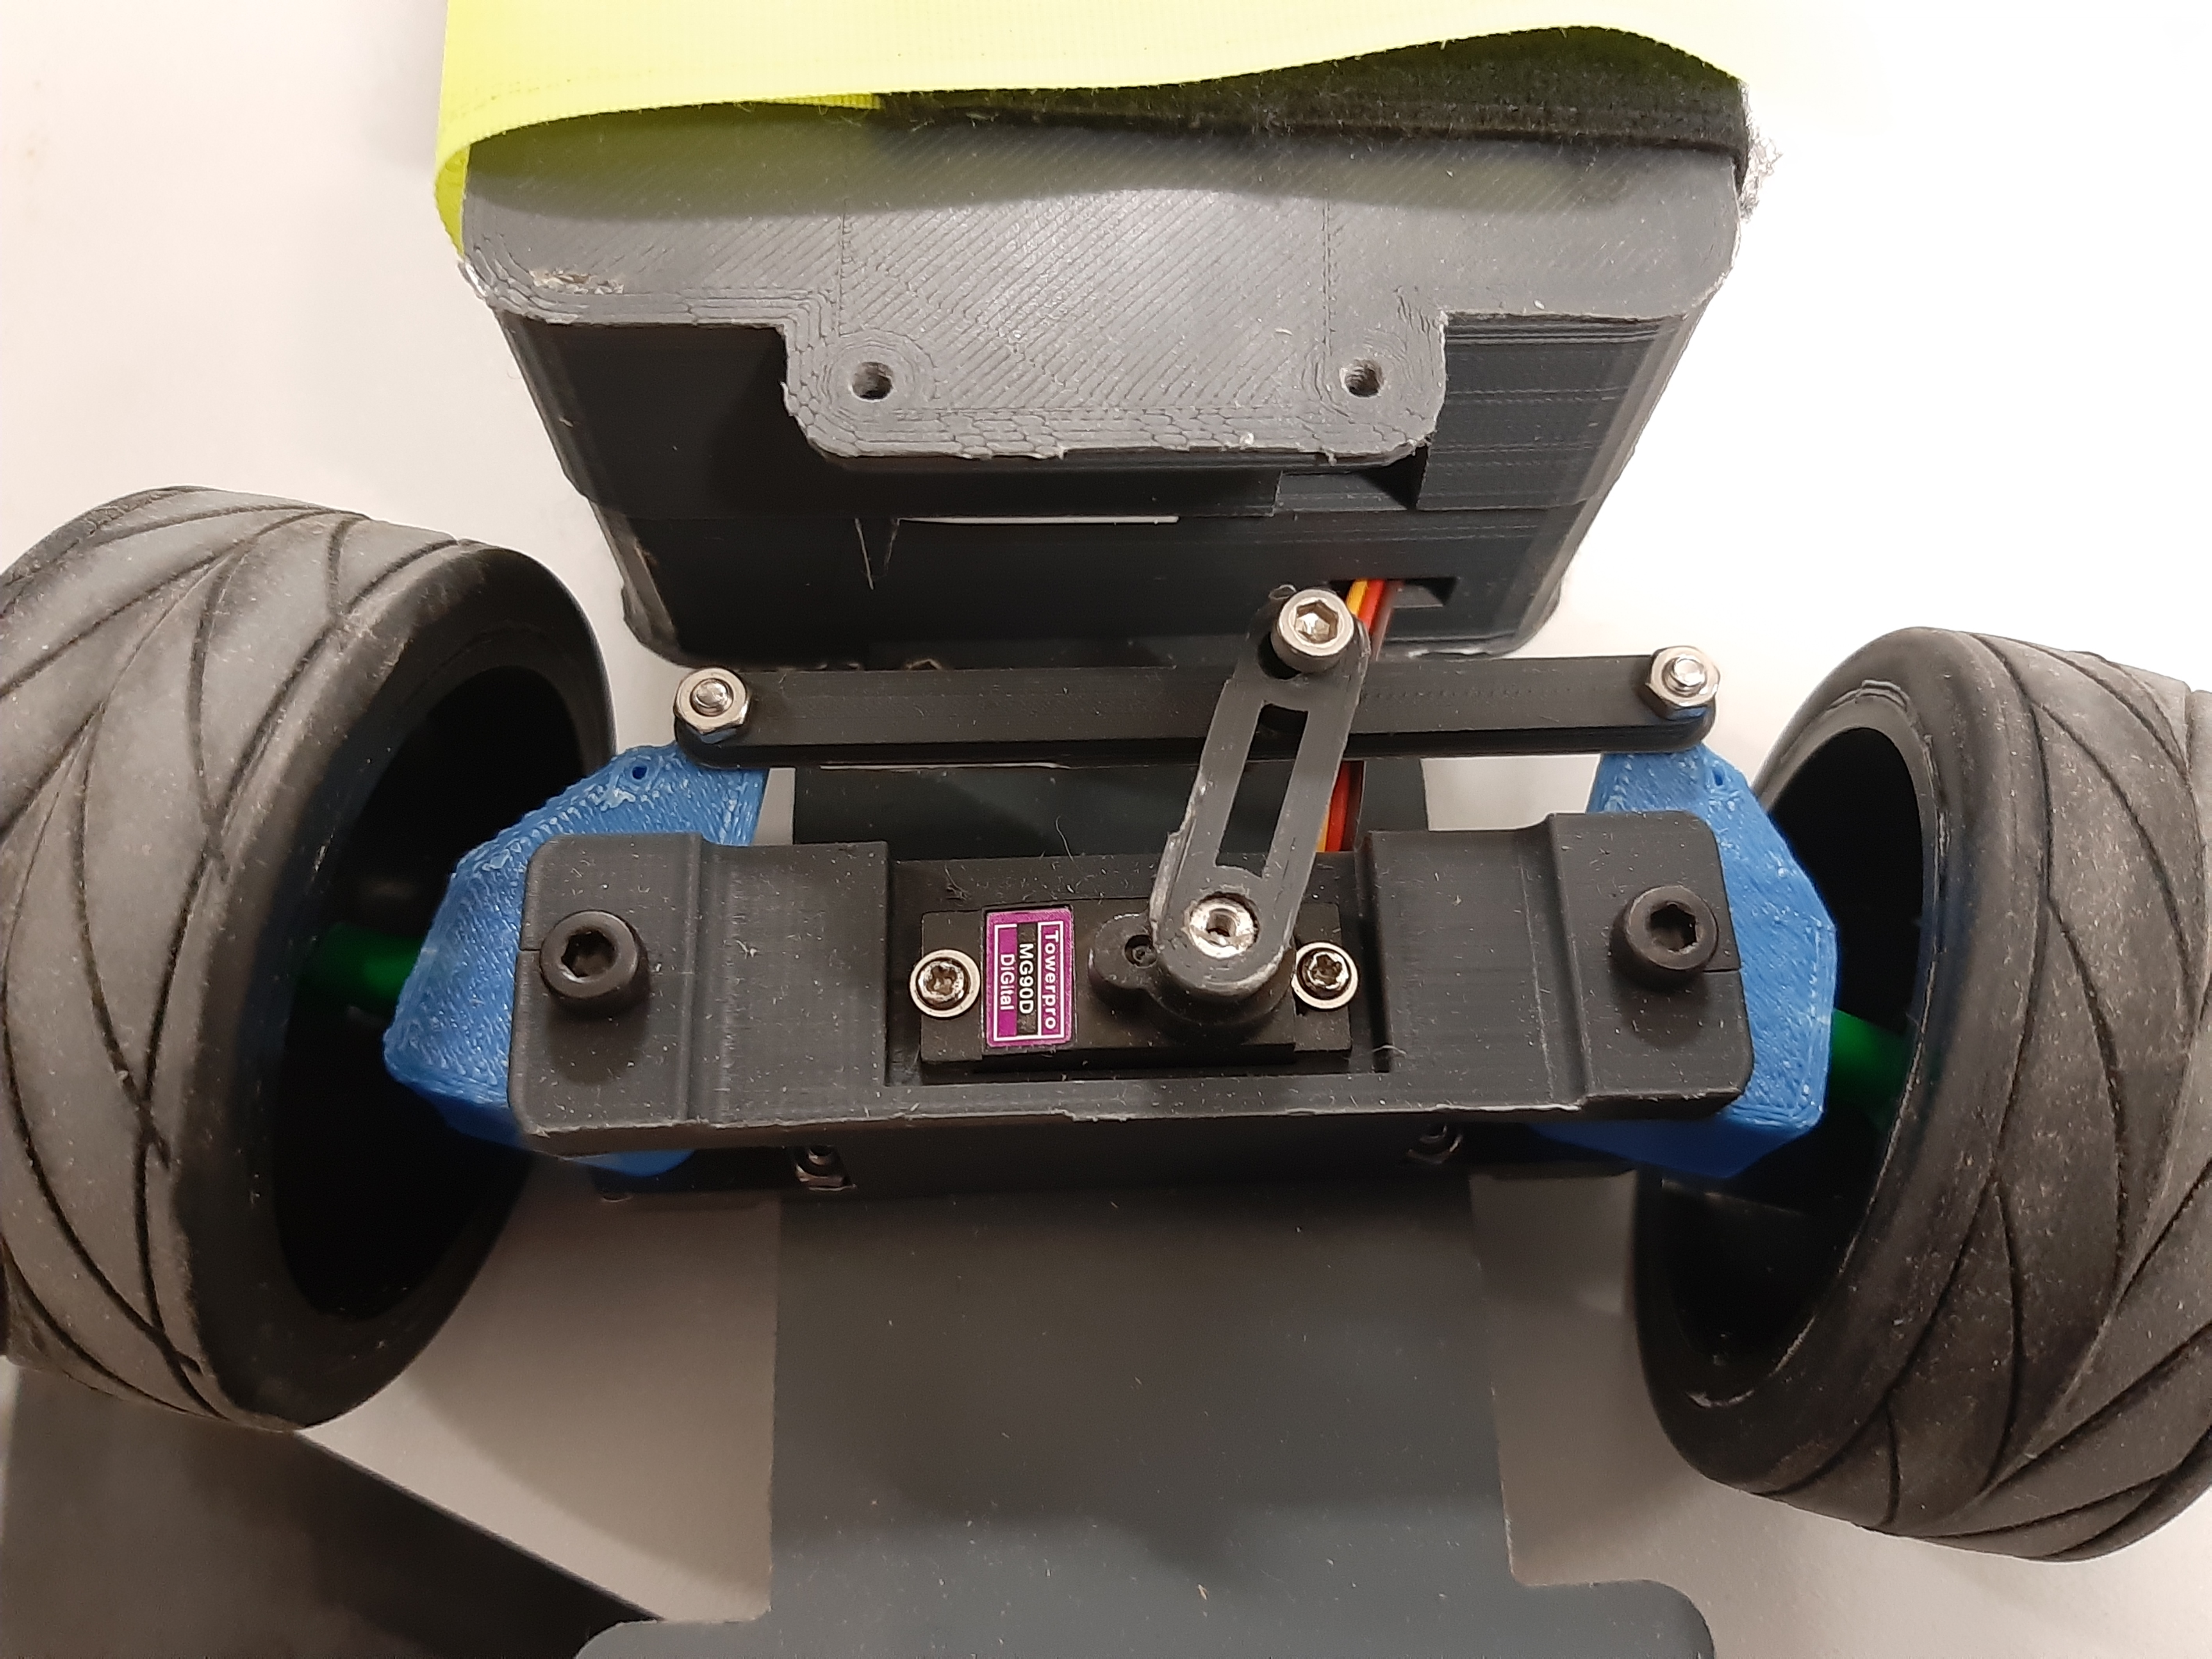
\includegraphics[width=\textwidth, height = 4cm]{vuav.jpg}
         \caption{L'avant du véhicule}
     \end{subfigure}
     ~
     \begin{subfigure}[b]{0.45\textwidth}
         \centering
         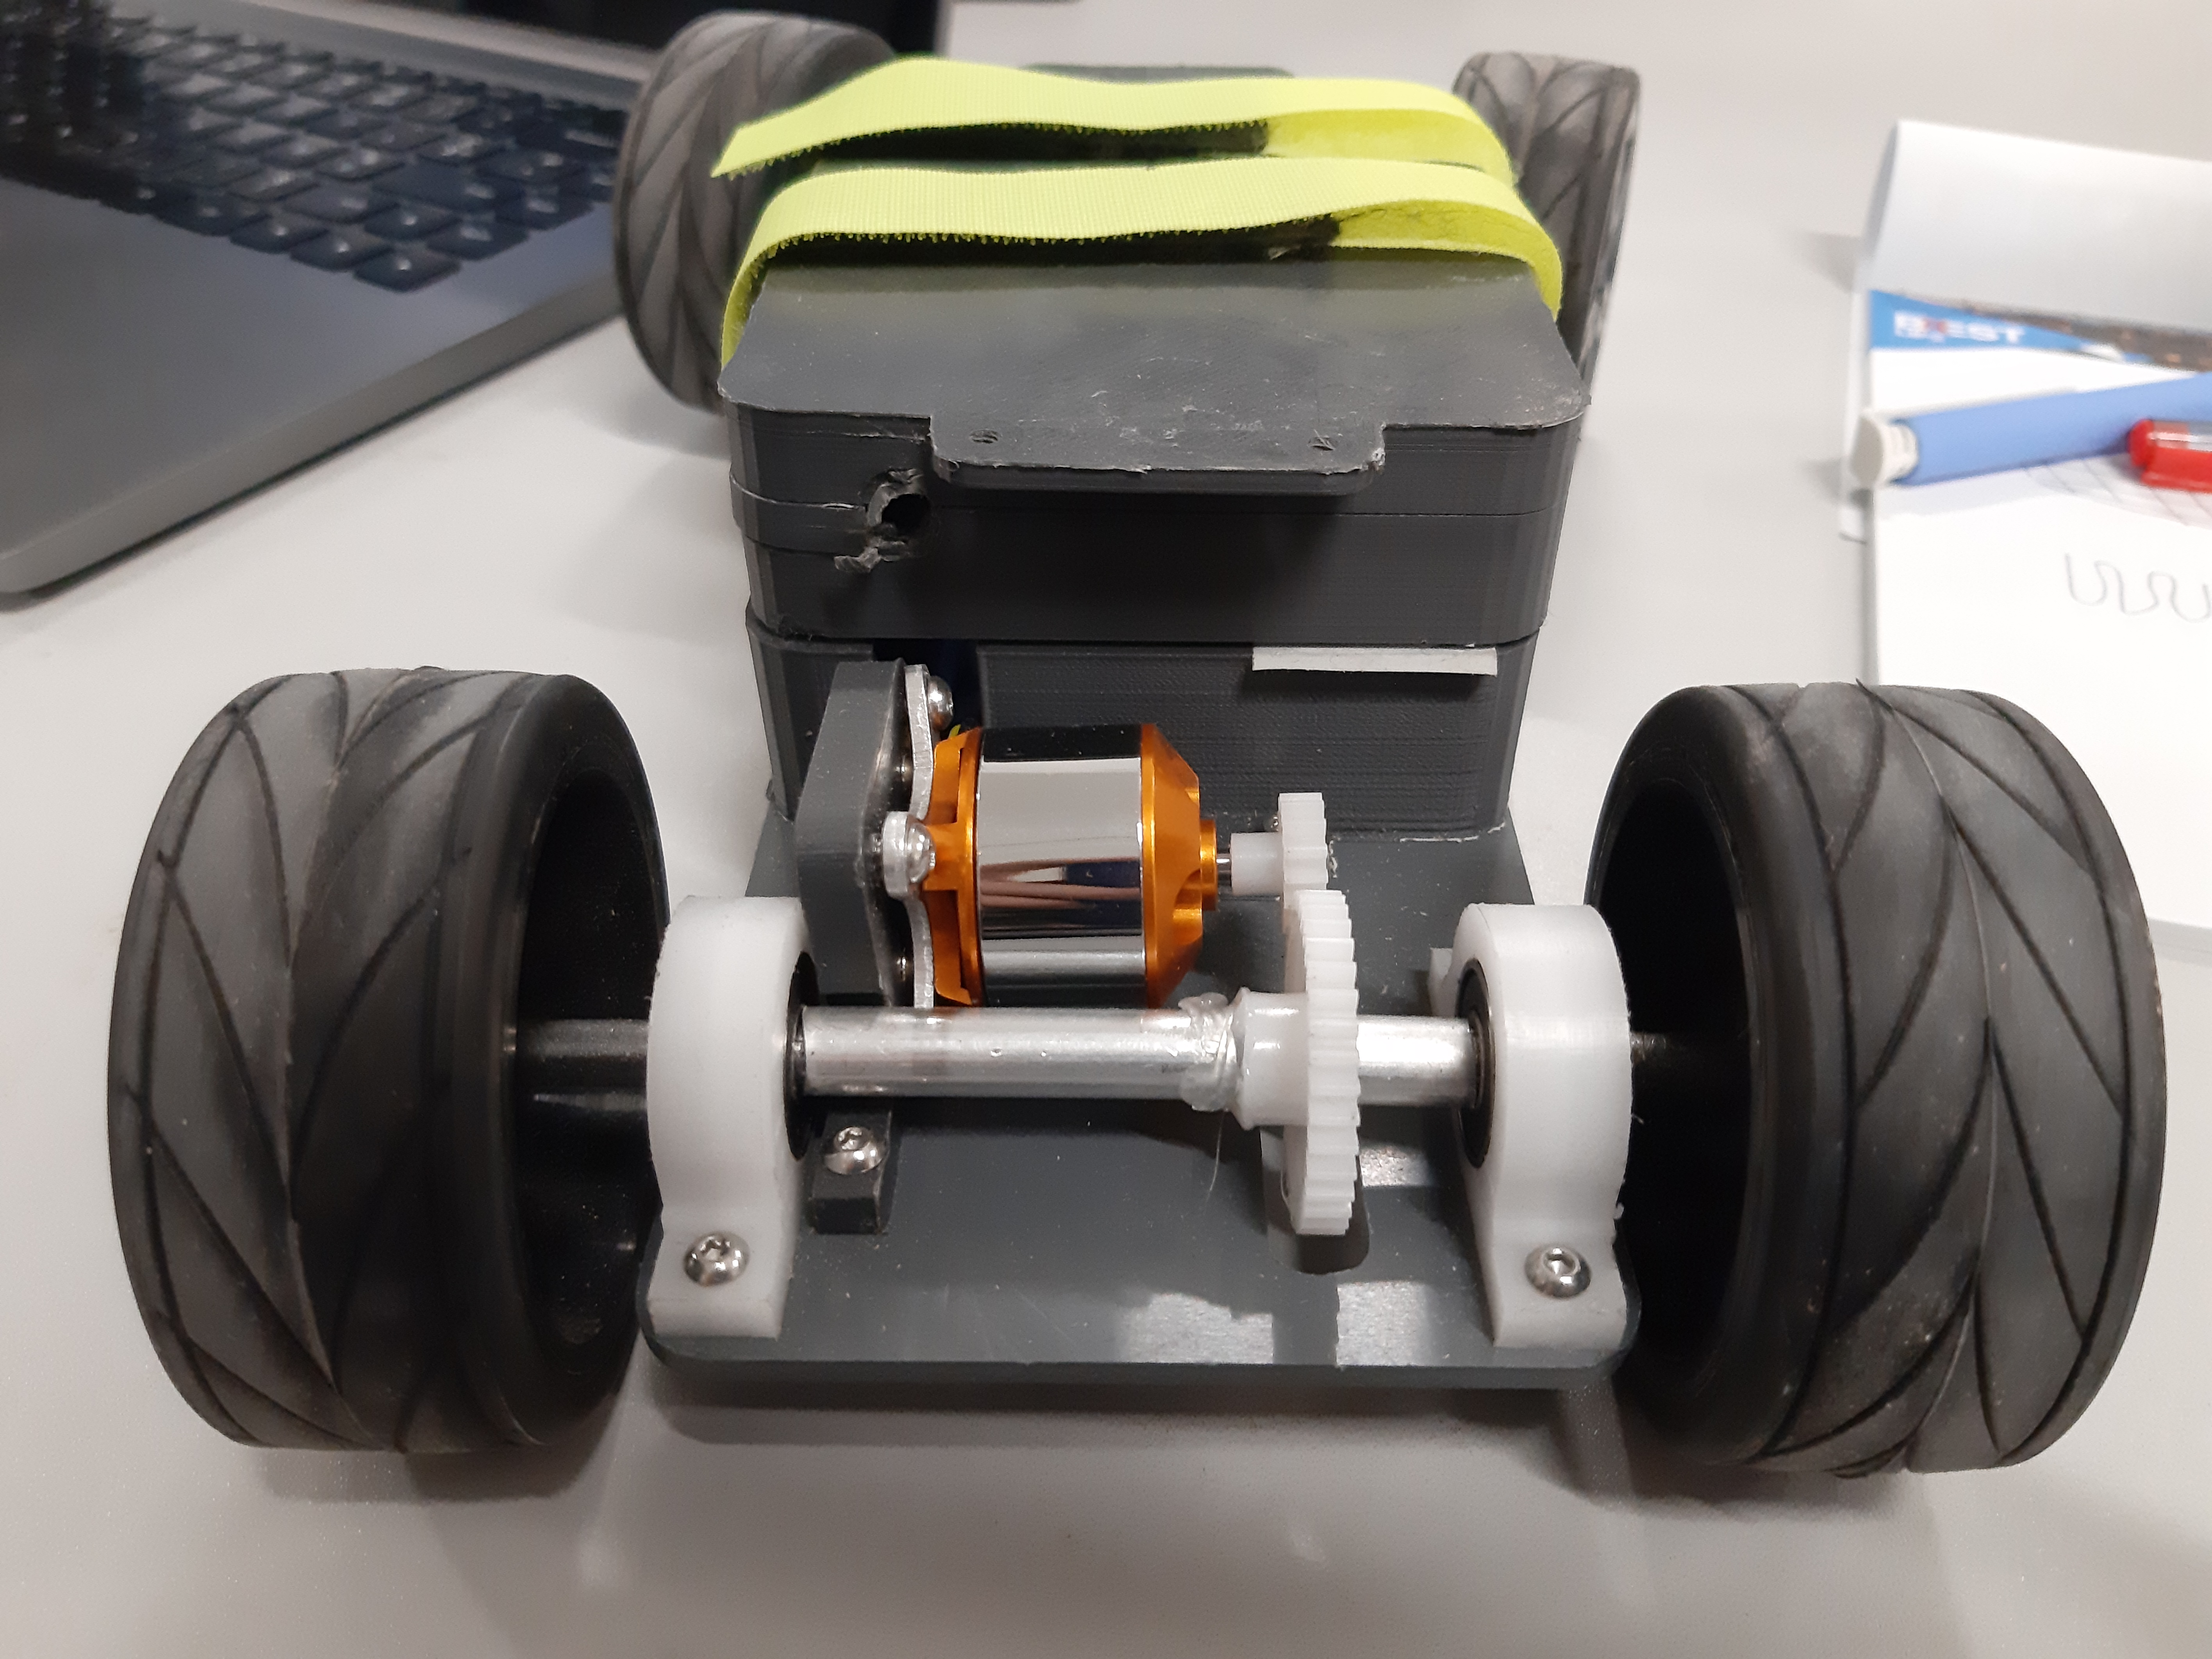
\includegraphics[width=\textwidth, height = 4cm]{vuar.jpg}
         \caption{L'arrière du véhicule}
     \end{subfigure}
     \caption{Zoom sur la voiture}
\end{figure}

Pour la partie électronique, la voiture a été équipée dans un premier temps d'une batterie, d'un moteur \textit{brushless}, d'un servomoteur et d'un récepteur pour la téléopération avec une télécommande. Différents tests ont été ensuite réalisés afin de vérifier la robustesse de la conception. Quelques problèmes ont été ainsi observés : le rapport de réduction était trop faible, et comme la voiture est très légère, il est très difficile de la conduire. Une solution à ce problème serait de rajouter un engrenage supplémentaire afin d'augmenter le rapport de réduction. Il est également envisageable d'augmenter la charge utile de la voiture (l'ajout des éléments nécessaires pour rendre le véhicule peut en effet résoudre ce problème, mais les tests n'ont pas été réalisés).\\

\subsection{Adaptation de l'architecture pour le projet}
Étant donné les solutions techniques choisies par l'équipe, une adaptation de l'architecture de la voiture s'impose :
\begin{itemize}[label=\textbullet, font=\small]
    \item Le traitement d'images et l'asservissement visuel est au coeur de notre solution. C'est pour cela que la conception d'un support caméra fiable est très importante. Le support conçu, permet ainsi de régler la position de la caméra mais également son angle d'inclinaison très rapidement sous \textit{Autodesk Inventor}. Nous avons désormais une solution de prototypage très rapide à fabriquer pour pouvoir mener les différents tests afin de trouver la meilleure position possible pour la caméra.
    \item Le support du capteur \textsc{GNSS} permet lui de surélever le capteur au dessus de la voiture afin d'éviter au maximum les interférences. Son positionnement est également réfléchi de telle sorte à ne pas trop déplacer le centre de gravité du véhicule vers l'arrière. Ceci est réalisé grâce au désaxage de la tige qui surélève le capteur. Sa proximité avec le support carte au milieu de la voiture, rend les branchements également plus simple.\\
\end{itemize}

\begin{figure}[H]
     \centering
     \begin{subfigure}[b]{0.45\textwidth}
         \centering
         \includegraphics[width=\textwidth, height = 5cm]{Support caméra.PNG}
         \caption{Support caméra}
     \end{subfigure}
     ~
     \begin{subfigure}[b]{0.45\textwidth}
         \centering
         \includegraphics[width=\textwidth, height = 5cm]{Support GPS.PNG}
         \caption{Support capteur \textsc{GNSS}}
     \end{subfigure}
     \caption{Pièces ajoutées}
     \label{fig:piece_aj}
\end{figure}

\section{Simulation sous \textsc{V-REP}}
\subsection{Modélisation de la voiture et du terrain}
Les circonstances actuelles ne nous permettent pas de travailler sur le projet en présentiel. La solution de repli qui a été adoptée est de construire une simulation de tout l'environnement du problème (voiture + terrain) afin de poursuivre le projet. Les outils de simulation permettent en effet de s'abstraire du matériel et de  valider des solutions techniques avant de les intégrer en réalité.\\

La simulation a été construite dans le cours de \textsc{M.Benoît Zerr}. Le tutoriel peut être consulté en suivant ce \href{https://www.ensta-bretagne.fr/zerr/dokuwiki/doku.php?id=vrep:main#v1}{lien}\footnote{https://www.ensta-bretagne.fr/zerr/dokuwiki/doku.php?id=vrep:main#v1}.\\

Le modèle dynamique est construit avec des formes simples (cylindres et parallélépipèdes) afin de réduire le temps de calcul lors de la simulation. Les pièces de la \textsc{CAO} ont été rajoutées par dessus afin d'avoir un aspect visuel qui permet de distinguer les différentes parties.\\

\begin{figure}[H]
     \centering
     \begin{subfigure}[b]{0.45\textwidth}
         \centering
         \includegraphics[width=\textwidth, height = 5cm]{mod_dyn.png}
         \caption{Modèle dynamique}
     \end{subfigure}
     ~
     \begin{subfigure}[b]{0.45\textwidth}
         \centering
         \includegraphics[width=\textwidth, height = 5cm]{mod_vis.png}
         \caption{Modèle graphique}
     \end{subfigure}
     \caption{Modélisation de la voiture}
     \label{fig:mod_dyn_vis}
\end{figure}

Dans le tutoriel précédent, il s'agit également de créer l'environnement dans lequel la voiture évoluera. Nous avons décidé de choisir comme revêtement de la route, une texture qui se rapproche le plus d'une vraie route. En effet, le traitement sur ce genre de texture est difficile compte tenu du bruit très élevé dans l'image : lignes pointillées, lignes doubles, bifurcations et le nombre de voies. Nous sommes partis du principe que si notre solution répond à la problématique sur une vraie route, il serait simple de l'adapter pour un usage sur une piste d'athlétisme.\\

\begin{figure}[H]
     \centering
     \includegraphics[width=8cm, height = 4cm]{route.png}
     \caption{Texture de la route}
     \label{fig:prob}
\end{figure}

\subsection{Modèle cinématique et interface avec \textsc{ROS}}
Sur la voiture, nous possédons deux commandes : l’accélération des roues arrières (qui sont motrices) et la vitesse de rotation du volant (servomoteur). Nous noterons $\delta$ l’angle entre les roues avant et l’axe de la voiture, et $\theta$ l’angle que fait la voiture par rapport à l’horizontale, et (x, y) les coordonnées du milieu de l’essieu arrière. Les variables d’état de notre système sont constituées par : 
\begin{itemize}[label=\textbullet, font=\small]
    \item \textbf{les coordonnées de position} : les coordonnées (x,y) du centre de l’essieu arrière, l’orientation $\theta$ de la voiture, et l’angle $\delta$ des roues avant ;
    \item \textbf{la coordonnée cinématique $\upsilon$} : représentant la vitesse du milieu de l’essieu avant (ceci est une approximation pour simplifier les équations : pour notre voiture, la vitesse est appliqué sur l'essieu arrière).
\end{itemize}
\begin{figure}[H]
     \centering
     \begin{subfigure}[b]{0.45\textwidth}
        \centering
            $$\left \{
            \begin{array}{c @{=} l}
                \dot{x}\ & \ \upsilon\, cos(\delta)\, cos(\theta) \\
                \dot{y}\ & \ \upsilon\, cos(\delta)\, sin(\theta) \\
                \dot{\theta}\ & \ \frac{\upsilon\, sin(\delta)}{L} \\
                \dot{\upsilon}\ & \ u_1 \\
                \dot{\delta}\ & \ u_2 
            \end{array}
            \right. $$
         \caption{Équations d'état}
     \end{subfigure}
     ~
     \begin{subfigure}[b]{0.45\textwidth}
         \centering
         \includegraphics[width=\textwidth, height = 5cm]{mod_cin.png}
         \caption{Modèle cinématique}
     \end{subfigure}
     \caption{Modélisation cinématique de la voiture}
     \label{fig:mod_dyn_vis}
\end{figure}

Nous avons ainsi deux variables à contrôler : 
\begin{itemize}[label=\textbullet, font=\small]
    \item \textbf{l’accélération des roues arrières $u_1$} : pour faire le lien avec la modélisation dynamique sous \textsc{V-REP}, cette commande doit correspondre à l'accélération des deux roues arrières. Mais pour simplifier le modèle et la simulation, nous allons considérer une vitesse $\upsilon$ constante. Ceci implique donc un changement dans les équations d'états :
            $$\left \{
            \begin{array}{c @{=} l}
                \dot{x}\ & \ \ u_1\, cos(\delta)\, cos(\theta) \\
                \dot{y}\ & \ \ u_1\, cos(\delta)\, sin(\theta) \\
                \dot{\theta}\ & \ \frac{\upsilon\, sin(\delta)}{L} \\
                \dot{\delta}\ & \ u_2 
            \end{array}
            \right. $$
    \item \textbf{la vitesse de rotation du volant $u_2$} : sur \textsc{V-REP}, cette commande va correspondre à la vitesse de rotation du servomoteur (en réalité, cette commande va contrôler deux liaisons pivots afin de simuler un servomoteur).\\
\end{itemize}

Le travail précédent nous permet ainsi de réaliser l'interface entre \textsc{ROS} et \textsc{V-REP} (en langage \textit{lua}). En plus des \textit{topics} relatifs aux deux commandes, nous avons également codé l'interface qui permet de simuler une caméra sur notre voiture. L'image obtenu est ainsi publiée sur un autre \textit{topic} afin d'être traitée dans un \textit{node} \textsc{ROS}.\\

\begin{figure}[H]
     \centering
     \includegraphics[width=\textwidth, height = 5cm]{topics.png}
     \caption{Interface entre ROS et V-REP}
     \label{fig:interface}
\end{figure}


\section{Drivers et nodes de bas-niveau sur la voiture}
En adéquation avec la simulation sous \textsc{V-REP}, nous avons développé des nodes \textsc{ROS} pour interfacer les différents capteurs et actionneurs.
\begin{figure}[H]
     \centering
     \includegraphics[width=13cm, height = 9cm]{Archi fonct info.PNG}
     \caption{Architecture fonctionnelle d'information}
     \label{fig:prob}
\end{figure}
Les drivers sont implémentés en utilisant le plus possible les nodes développés par la communauté ROS. Le GNSS et l'IMU sont représentés mais à notre stade d'avance de ce projet, ils ne sont pas utilisés.
Le package \textit{cv\_camera} nous permet de publier une image sur un topic ROS issue
de la caméra de la Raspberry pi.
Pour l’envoi de signaux PWM vers l’ESC et le servo de direction, nous avons développé
un node Python utilisant une bibliothèque pour contrôler la carte Maestro via la
connexion série USB. Ce dernier node s'abonne aux mêmes topics que notre simulation \textsc{V-REP} pour permettre à terme de faire du \textit{Hardware in the loop}.



\section{Pipeline de contrôle}
Désormais, nous avons tous les éléments nécessaires afin de rendre la voiture autonome. Dans cette partie, nous allons détailler la \textit{pipeline de contrôle} : d'une \textit{frame} issue de la caméra jusqu'au calcul de $u_1$ et $u_2$.
\subsection{Autour du suivi de lignes}
Depuis quelques années, de nombreux chercheurs travaillent sur
des projets concernant l'aide à la conduite automobile par vision
artificielle. Beaucoup de projets ont vu le jour et les techniques développées sont très variées.\\

Deux approches peuvent répondre à notre problématique :
\begin{itemize}[label=\textbullet, font=\small]
    \item Positionner la voiture sur une ligne de la piste et faire en sorte de suivre cette ligne en la gardant toujours au milieu sous le châssis de la voiture. Cette approche peut s'avérer efficace pour faire uniquement un suivi de ligne. Cependant, nous avons vu quelques inconvénients à utiliser cette méthode : d'abord la largeur de la ligne blanche de la piste mesure un peu plus de la moitié de la largeur du châssis de la voiture (5cm). Ceci pourrait poser un soucis si la focale de la caméra n'est pas suffisamment petite (on aurait une image presque toute blanche, ce qui compliquerait la détection et le contrôle). De plus, les algorithmes à développer ne serviront pas à d'autres situation (conduite en milieu urbain par exemple). En revanche, cette méthode fonctionne très bien en simulation.
    \item Positionner la voiture sur une voie de la route et détecter les deux lignes délimitant cette voie. Cette méthode se rapproche un peu plus de ce qui se fait dans l'industrie automobile en terme de conduite autonome (cf voiture autonome \textit{Tesla}). Nous avons donc opté pour cette deuxième solution.
\end{itemize}

\subsection{Les étapes de la pipeline}
\begin{figure}[H]
     \centering
     \includegraphics[scale = 0.67]{pipeline.png}
     \caption{Pipeline de contrôle}
     \label{fig:pipeline}
\end{figure}
\pagebreak

\subsubsection{Prétraitement}
\begin{enumerate}
    \item \textbf{Bird Eye View} : cette vue permet d'opérer une transformation de l'image source afin d'avoir une perspective de la route. Elle règle le problème des lignes parallèles qui se coupent à l'horizon par exemple.
\begin{figure}[H]
     \centering
     \begin{subfigure}[b]{0.4\textwidth}
         \centering
         \includegraphics[width=\textwidth, height = 3.5cm]{image.png}
         \caption{Image Source}
     \end{subfigure}
     ~
     \begin{subfigure}[b]{0.4\textwidth}
         \centering
         \includegraphics[width=\textwidth, height = 3.5cm]{birdView.png}
         \caption{Bird Eye View}
     \end{subfigure}
     \\
     \begin{subfigure}[b]{0.4\textwidth}
         \centering
         \includegraphics[width=\textwidth, height = 3.5cm]{virageD.png}
         \caption{Image Source}
     \end{subfigure}
     ~
     \begin{subfigure}[b]{0.4\textwidth}
         \centering
         \includegraphics[width=\textwidth, height = 3.5cm]{birdVie1.png}
         \caption{Bird Eye View}
     \end{subfigure}
     \caption{Bird Eye View}
     \label{fig:bev}     
\end{figure}
    \item \textbf{Extraction des régions d'intérêt} : cette étape permet de diviser l'image issue de l'étape précédente en deux régions : gauche et droite.
    \item \textbf{Filtrage} : on applique deux filtres différents pour les deux régions afin d'extraire les \textit{pixels} qui nous intéresse. En effet, la ligne gauche de la voie est complètement différente de celle de droite (ligne double jaune, ligne en pointillées blanches).
\end{enumerate}

À la fin de cette étape, nous avons filtré l'image de la route et elle est donc prête pour l'étape suivante.

\begin{figure}[H]
     \centering
     \begin{subfigure}[b]{0.45\textwidth}
         \centering
         \includegraphics[width=\textwidth, height = 3.5cm]{5.png}
         \caption{Image Source}
     \end{subfigure}
     \\
     \begin{subfigure}[b]{0.45\textwidth}
         \centering
         \includegraphics[width=\textwidth, height = 3.5cm]{roiL.png}
         \caption{Bird Eye View}
     \end{subfigure}
     ~
     \begin{subfigure}[b]{0.45\textwidth}
         \centering
         \includegraphics[width=\textwidth, height = 3.5cm]{roiR.png}
         \caption{Image Source}
     \end{subfigure}
    \caption{Extraction des RoI}
    \label{fig:roi} 
\end{figure}

\subsubsection{\textit{Full Search}}
Cette algorithme a pour objectif de détecter les \textit{pixels} qui constituent chaque ligne.
\begin{enumerate}
    \item \textbf{Détection} : on divise l'image issue de la précédente étape en $n$ sous-fenêtres. Ensuite, on parcourt avec deux indices l'image (indices sur x) : un qui part de 0 vers la droite, et l'autre de la droite (largeur de l'image) vers la gauche. À chaque itération, on retient les deux indices uniquement s'ils sont à l'intérieur de la fenêtre (limitée par deux indices sur $y$), auquel cas on calcule la somme des \textit{pixels} blancs sur les colonnes données par chacun de ces indices. Si cette somme est supérieure à un seuil, on arrête d'itérer. À la fin de la boucle, on obtient un encadrement de notre ligne avec deux listes d'indices.
    \item \textbf{Interpolation} : avec les deux listes précédentes, on effectue une interpolation polynomiale pour approximer la ligne avec un polynôme du second degré. On obtient ainsi les coefficients de ce polynôme.
\end{enumerate}
\begin{figure}[H]
     \centering
     \begin{subfigure}[b]{0.4\textwidth}
         \centering
         \includegraphics[width=\textwidth, height = 3.5cm]{3.png}
         \caption{Image Source}
     \end{subfigure}
     ~
     \begin{subfigure}[b]{0.4\textwidth}
         \centering
         \includegraphics[width=\textwidth, height = 3.5cm]{fs.png}
         \caption{Interpolation}
     \end{subfigure}
     \\
     \begin{subfigure}[b]{0.4\textwidth}
         \centering
         \includegraphics[width=\textwidth, height = 3.5cm]{5.png}
         \caption{Image Source}
     \end{subfigure}
     ~
     \begin{subfigure}[b]{0.4\textwidth}
         \centering
         \includegraphics[width=\textwidth, height = 3.5cm]{fs2.png}
         \caption{Interpolation}
     \end{subfigure}
     \caption{Détection de la voie}
     \label{fig:detect}     
\end{figure}

\subsubsection{Post-traitement}
Cette étape permet d'extraire les informations qui nous permettront de contrôler la voiture. Grâce à l'étape précédente et à l'interpolation polynomiale, nous pouvons proposer une nouvelle méthode pour contrôler la voiture :  
\begin{enumerate}
    \item \textbf{Décalage par rapport au centre de la voie} : on fait un calcul supplémentaire pour déterminer la position de la voiture dans l'image (en exploitant la présence du capot dans l'image brute notamment). Une fois cette position connue, on calcul le décalage de la voiture par rapport au centre de la voie : en fonction de la détection de la ligne de gauche et de droite, on arrive à calculer avec précision cette donnée. Le décalage par rapport au centre est ensuite utilisé pour alimenter le \textit{node} de contrôle qui calcule l'angle à appliquer sur les roues afin de rester au milieu de la voie.
    \item \textbf{Rayon de courbure} : nous calculons également le rayon de courbure de la voie. Ceci nous permet de savoir dans quel sens on tourne mais également d'adapter la vitesse de la voiture. Plus le rayon de courbure devient petit, plus le virage est serré. Il faut donc réduire la vitesse de la voiture. Pour l'instant, cette donnée n'est pas exploité dans la suite. En effet, comme il s'agit d'un calcul de dérivée, la donnée brute est trop bruitée. Il faut ainsi appliquer un filtre pour l'exploiter.
\end{enumerate}
\begin{figure}[H]
     \centering
     \begin{subfigure}[b]{\textwidth}
         \centering
         \includegraphics[width=\textwidth, height = 4cm]{visual.png}
         \caption{Road status 1}
     \end{subfigure}
     \\
     \begin{subfigure}[b]{\textwidth}
         \centering
         \includegraphics[width=\textwidth, height = 4cm]{visualoffG.png}
         \caption{Road status 2}
     \end{subfigure}
     \caption{Résultat de la pipeline}
     \label{fig:res}     
\end{figure}

\subsubsection{Noeud de contrôle}
Nous avons utilisé comme interface de contrôle \textit{rqt} afin de publier un message contenant la vitesse de la voiture. Le package \textit{PID} de \textsc{ROS} a été également utilisé afin de fournir les commandes $u_1$ et $u_2$. Ce noeud est simplement lancé dans le fichier \textit{.launch} après une opération de \textit{remap} pour rediriger les topics \textsc{ROS} correspondants.

\begin{figure}[H]
     \centering
         \includegraphics[width=\textwidth, height = 4cm]{inter_ctrl.png}
        \caption{Interface de contrôle}
        \label{fig:res}     
\end{figure}

\section{Résultats}
Le traitement précédent n'a été testé qu'en simulation, cependant les résultats obtenus sont prometteurs quant à son utilisation sur un terrain réel : la voiture arrive à faire le tour du terrain de façon autonome.\\

Un lien d'une vidéo de démonstration est disponible sur le dépôt \textit{GitHub} du projet.

\begin{figure}[H]
     \centering
         \includegraphics[width=\textwidth, height = 9.5cm]{test_res.png}
        \caption{Interface V-REP}
        \label{fig:res}     
\end{figure}

\section{Perspectives d'améliorations}
D'un point de vue mécanique, nous avions parlé du problème lié à la réduction de vitesse en sortie du moteur qui n'était pas assez grande et qui rendait le contrôle de la voiture difficile. Ceci pourrait être réglé en ajoutant étage de réduction avec un autre engrenage. Pour cela vu le peu de place restant à l'arrière de la voiture, il faudrait redessiner tout le système de réduction pour pouvoir rajouter cet engrenage.\\

Pour ce qui est du poids de la voiture, les tests effectués avec des poids à l'avant de la voiture étaient relativement concluant. Il faudrait d'abord assembler tous les capteurs et toutes les pièces mécaniques avant de décider si il est nécessaire d'alourdir la voiture ou non.\\

Concernant l'utilisation du capteur GNSS et de la centrale inertielle, nous avons délibérément choisi de ne pas les utiliser et d'effectuer seulement l'asservissement via le suivi de ligne. Comme améliorations possibles nous pourrions ainsi rajouter une odométrie visuelle avec la caméra et fusionner cette donnée avec celle du capteur GNSS et de la centrale inertielle afin d'avoir l'état complet de la voiture.\\ 

<<<<<<< HEAD
Pour la partie asservissement visuel, nous sommes encore loin d'atteindre des résultats fiables et robustes. En effet, quelques problèmes sont d'ores et déjà réglés comme la non détection des lignes sur une frame. Cependant, beaucoup d'améliorations restent à faire :
\begin{itemize}[label=\textbullet, font=\small]
    \item Effectuer un \textit{FullSearch} uniquement sur la première frame. Ensuite, au lieu de rechercher les lignes de la voie sur toute l'image, on recherche uniquement dans une zone proche de la zone ou la détection s'est effectué sur l'image d'avant. L'implémentation de la librairie qui effectue la pipeline de contrôle en orienté objet permettrait de passer facilement à cette étape ;
    \item Comme mentionné précédemment, le rayon de courbure n'est pas utilisé pour l'instant. Il faudrait implémenter un filtre afin d'exploiter cette donnée ;
    \item Comme dernière étape, au lieu d'extraire les deux régions en bas de l'image, on peut lancer la détection sur toute l'image. Cela pourrait améliorer le calcul du rayon de courbure. Mais pour cela, il faut trouver les bons filtres et prétraitements à appliquer.\\ 
\end{itemize}

Enfin, après avoir suivi les cours de systèmes embarqués, nous comprenons que le fait d'utiliser un \textit{Linux} classique (comme \textit{Ubuntu}) n'est pas la solution optimale pour une \textit{Raspberry}. L'utilisation de Buildroot afin de concevoir et de compiler directement les briques élémentaires composant notre Linux embarqué, est un complément qui serait très intéressant. Nous ne savons pas si cela rendrait l'exécution des codes plus rapides, mais il serait bien de pouvoir comparer ces deux solutions différentes afin de choisir la meilleure des deux.\\
=======
\section{Perspectives et améliorations}
--> Mettre toutes les améliorations possibles (Docker)
>>>>>>> b5d2ff851ae198be8a7444f66db44fb074a962ed

\section*{Conclusion}
\addcontentsline{toc}{chapter}{Conclusion}
Pour conclure, ce projet nous a permis de mettre en pratique différents cours étudiés durant cette année, tels que ceux de \textit{ROS}, de \textit{Traitement d'image}, de \textit{VREP} ou même de \textit{Conception et réalisation}. Il s'apparente comme étant une synthèse de nos connaissances et permet à juste titre de faire le point sur nos compétences et nos capacités en tant que futur ingénieur roboticien.\\
\pagebreak

<<<<<<< HEAD
\begin{appendix}
    \chapter{Complément Architecture Électronique}
    \label{carchf}
Le schéma suivant permet de valider le choix des capteurs, des adaptateurs de tension ainsi que des contrôleurs.\\
\begin{figure}[H]
     \centering
     \includegraphics[width=13cm, height = 9cm]{Archi fonct tension.png}
     \caption{Architecture fonctionnelle d'alimentation}
     \label{fig:arch_compl}
\end{figure}
\end{appendix}
=======
\section*{Annexe1 : Raspberry comme ordinateur de bord}
\addcontentsline{toc}{chapter}{Annexe1}

Nous avons choisi d'installer Raspbian sur notre raspberry, cela nous permet d'avoir un accès simple à la caméra, cependant l'installation de ROS est un peu plus longue, car il faut recompiler les sources.

Pour installer ROS sur notre raspberry pi 3 nous avons suivi la documentation officielle :  \url{http://wiki.ros.org/ROSberryPi/Installing%20ROS%20Kinetic%20on%20the%20Raspberry%20Pi}


>>>>>>> b5d2ff851ae198be8a7444f66db44fb074a962ed

\pagebreak
\listoffigures
\end{document}

